\documentclass[11pt]{beamer}
\usepackage{graphicx}
\graphicspath{ {./Images/} }
\setbeamertemplate{caption}[numbered]
\usepackage{caption}
\usepackage{float}
\usepackage{hyperref}
\usepackage{multirow}
\setbeamersize{text margin left=0.5cm, text margin right=0.5cm}
\usepackage{multicol}
\usepackage{listings}
\usepackage{color}
\usepackage{fancyvrb}
\usepackage{booktabs}
\definecolor{dkgreen}{rgb}{0,0.6,0}
\definecolor{gray}{rgb}{0.5,0.5,0.5}
\definecolor{mauve}{rgb}{0.58,0,0.82}
\lstset{
    language=Java,
    frame=single,
    aboveskip=3mm,
    belowskip=3mm,
    showstringspaces=false,
    columns=flexible,
    basicstyle={\small\ttfamily},
    numbers=none,
    numberstyle=\tiny\color{gray},
    keywordstyle=\color{blue},
    commentstyle=\color{dkgreen},
    stringstyle=\color{mauve},
    breaklines=true,
    breakatwhitespace=true,
    tabsize=3
    }

\makeatletter
\let\save@measuring@true\measuring@true
\def\measuring@true{
    \save@measuring@true
    \def\beamer@sortzero##1{\beamer@ifnextcharospec{\beamer@sortzeroread{##1}}{}}%
    \def\beamer@sortzeroread##1<##2>{}
    \def\beamer@finalnospec{}
    }
\makeatother
\mode<presentation> {
    \usetheme{Warsaw}
    \setbeamertemplate{footline}[page number]
    }
\definecolor{violet}{rgb}{0.54, 0.17, 0.89}
\newcommand{\red}[1]{\textcolor{red}{#1}}
\newcommand{\violet}[1]{\textcolor{violet}{#1}}
\newcommand{\green}[1]{\textcolor{green}{#1}}
\newcommand{\sol}{\textbf{Solution}: \pause \newline}

\title[Chapter 02 Notes]{Math 130: Introduction to Programming \\ Chapter 02: Java Fundamentals \\ Lecture Notes}
\author{
    Jesús R. Pérez Cuarenta \\
    \href{mailto:jperezcuarenta@swccd.edu}{jperezcuarenta@swccd.edu}
    }
\date{}

\begin{document}
  \section{}
  \begin{frame}
    \maketitle
  \end{frame}

  \begin{frame}
    \begin{multicols}{2}
        \tableofcontents
        \end{multicols}
  \end{frame}

\section{Basics}
\subsection{The Parts of a Java Program}
\begin{frame}[fragile]{The Parts of a Java Program}
    Java programs are made up of different parts. \\ \vspace{1em}
    Your first step in learning Java is to learn what the parts are. \\ \vspace{1em}
    Here is an example of a Java program:
    \begin{lstlisting}
public class HelloWorld {
    public static void main(String[] args) {
        System.out.println("Hello world!");
        }
    }
    \end{lstlisting}
\end{frame}

\begin{frame}[fragile]{The Parts of a Java Program}
    Here is a dissection of what statements mean in a simple Java program.
    \noindent
    \begin{figure}[H]
    \centering
    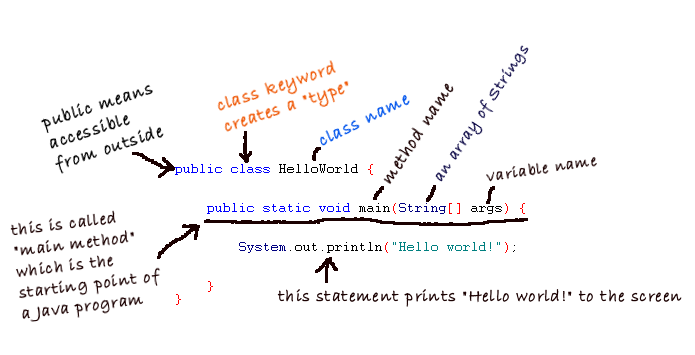
\includegraphics[scale=0.5]{Images/chapter02_section01_01.png}
    \end{figure}
\end{frame}

\begin{frame}[fragile]{The Parts of a Java Program}
    Assume the previous program is contained in a file called \texttt{HelloWorld.java} (it's just text after all, right?). \\ \vspace{1em}
    It may be compiled with the command \texttt{javac HelloWorld.java}. \\ \vspace{1em}
    The compiler creates another file named \texttt{HelloWorld.class}, which contains the translated Java byte code. \\ \vspace{1em}
    The \texttt{class} file can be executed with the command \texttt{java HelloWorld}.
\end{frame}

\subsection{The \texttt{print} Methods, and the Java API}
\begin{frame}[fragile]{The \texttt{print} and \texttt{println} Methods}
    The \texttt{print} and \texttt{println} \violet{methods} are used to display text output. \\ \vspace{1em}
    Performing output in Java, as well as many other tasks, is accomplished by using the Java API (Application Programmer Interface). \\ \vspace{1em}
    The \red{API} is a standard library of \red{prewritten classes} for performing specific operations. \\ \vspace{1em}
    The \texttt{print} and \texttt{println} \violet{methods} are part of the API and provide ways for output to be displayed on the standard output device.
\end{frame}

\begin{frame}[fragile]{The \texttt{print} and \texttt{println} Methods}
    \texttt{System} is a \violet{class} that is part of the Java API. \\ \vspace{1em}
    The \texttt{System} \violet{class} contains \violet{objects} and \violet{methods} that perform system-level operations. \\ \vspace{1em}
     One of the \violet{objects} contained in the \texttt{System} \violet{class} is named \texttt{out}. \\ \vspace{1em}
     The \texttt{out} \violet{object} has \violet{methods}, such as \texttt{print} and \texttt{println} , for performing output on the system console, or standard output device.
\end{frame}

\begin{frame}[fragile]{The \texttt{print} and \texttt{println} Methods}
    \noindent 
    \begin{figure}[H]
    \centering
    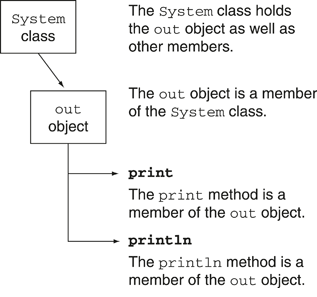
\includegraphics[scale=0.8]{Images/chapter02_section02_01.png}
    \end{figure}
\end{frame}

\begin{frame}[fragile]{The \texttt{print} and \texttt{println} Methods}
    The value that is to be displayed on the screen is placed inside the parentheses of the \texttt{print} \violet{methods}. \\ \vspace{1em}
    This value is known as an argument. \\ \vspace{1em}
    The following statement executes the \texttt{println} \violet{method} using the \violet{string} `'King Arthur'' as its argument. \\ \vspace{1em}
    \begin{lstlisting}
    System.out.println("King Arthur");
    \end{lstlisting}
    Note: The quotation marks are not displayed.
\end{frame}

\begin{frame}[fragile]{The \texttt{print} and \texttt{println} Methods}
    The difference between \texttt{print} and \texttt{println} is that the latter advances the cursor to the beginning of the next line.
    \begin{lstlisting}
    // TwoLines.java
    public class TwoLines {
        public static void main(String[] args) {
            System.out.println("A: I am here.");
            System.out.print("B: I am in the next line. ");
            System.out.print("C: Still on the same line.");
            }
        }
    \end{lstlisting}
    Note: The green line is a comment due to the two forward slashes. Comments are not executed by Java, they instead help leave notes behind for the sake of readability.
\end{frame}

\begin{frame}[fragile]{The \texttt{print} and \texttt{println} Methods}
    An alternative to \texttt{println} is to use an \red{escape sequence}. \\ \vspace{1em}
    An \red{escape sequence} starts with the backslash character ($\backslash$) and is followed by one or more \red{control characters}. \\ \vspace{1em}
    The \red{escape sequence} that causes the output cursor to go to the next line is \texttt{$\backslash$n}.
    \begin{lstlisting}
    // Adjusted.java
    public class Adjusted {
        public static void main(String[] args) {
            System.out.print("These are our top sellers:\n");
            System.out.print("Computer games\nCoffee\n");
            System.out.println("Aspirin");
            }
        }
    \end{lstlisting}
\end{frame}

\section{Data}
\subsection{Variables and Literals}
\begin{frame}[fragile]{Variables and Literals}
    A \violet{variable} is a named storage location in the computer's memory. \\ \vspace{1em} 
    A \violet{literal} is a value that is written into the code of a program. \\ \vspace{1em}
    Let's start with a program:
    \begin{lstlisting}
    // Variable.java
    public class Variable {
        public static void main(String[] args) {
            int value;
            value = 5;
            System.out.print("The value is ");
            System.out.println(value);
            }
        }
    \end{lstlisting}
\end{frame}

\begin{frame}[fragile]{Variables and Literals}
    The following statement is called a \texttt{\violet{variable} declaration}.
    \begin{lstlisting}
    int value;
    \end{lstlisting}
    A \violet{variable} declaration tells the compiler the \violet{variable's} name and the type of data it will hold. \\ \vspace{1em}
    This line indicates the \violet{variable's} name is \texttt{value}. \\ \vspace{1em} 
    The word \texttt{int} stands for integer, so \texttt{value} will only be used to hold integer numbers. \\ \vspace{1em} 
    Notice that \violet{variable} declarations end with a semicolon.
\end{frame}

\begin{frame}[fragile]{Variables and Literals}
    The following is called an \texttt{assignment statement}.
    \begin{lstlisting}
    value = 5;
    \end{lstlisting}
    The equal sign is an operator that stores the value on its right (in this case 5) into the \violet{variable} named on its left. \\ \vspace{1em} 
    After this line executes, the \texttt{value} \violet{variable} will contain the value 5.
\end{frame}

\begin{frame}[fragile]{Variables and Literals}
    Now consider the following statements
    \begin{lstlisting}
    System.out.print("The value is ");
    System.out.println(value);
    \end{lstlisting}
    The first statement sends the \violet{string literal} ``The value is'' to the \texttt{print} \violet{method}. \\ \vspace{1em}
    The next statement sends the name of the \texttt{value} variable to the \texttt{println} \violet{method}. \\ \vspace{1em} 
    When you send a \violet{variable} name to \texttt{print} or \texttt{println}, the \violet{variable's} contents are displayed. \\ \vspace{1em}
    Notice there are no quotation marks around \texttt{value}.
\end{frame}


\begin{frame}[fragile]{Variables and Literals}
    Look at a similar program that uses quotation marks around a \violet{variable}.
    \begin{lstlisting}
    // Variable02.java
    public class Variable02 {
        public static void main(String[] args) {
            int value;
            value = 5;
            System.out.print("The value is ");
            System.out.println("value");
            }
        }
    \end{lstlisting}
    When double quotation marks are placed around the word value it becomes a \violet{string literal}.
\end{frame}

\begin{frame}[fragile]{Variables and Literals}
    When the + operator is used with \violet{strings}, it is known as the \violet{string concatenation} operator. \\ \vspace{1em}
    The statement
    \begin{lstlisting}
    System.out.println("This is " + "one string.");
    \end{lstlisting}
    will print: This is one string. \\ \vspace{1em}
    You can also use the + operator to concatenate the contents of a \violet{variable} to a \violet{string}.
    \begin{lstlisting}
    number = 5;
    System.out.println("The value is " + number);
    \end{lstlisting}
    Although \texttt{number} is not a \violet{string}, the + operator converts its value to a \violet{string} and then concatenates, displaying: The value is 5.
\end{frame}

\begin{frame}[fragile]{Variables and Literals}
    An \texttt{identifier} is a programmer-defined name that represents some element of a program. \\ \vspace{1em}
    \violet{Variable} names and \violet{class} names are examples of identifiers. \\ \vspace{1em}
    You may choose your own \violet{variable} names and class names in Java, as long as you do not ue any of the Java key words. \\ \vspace{1em}
    Put some thought into the names assigned to your variables:
    \begin{lstlisting}
    int x; // hard to understand what _x_ represents
    int itemsOrdered; // a quantity associated to ordered items
    \end{lstlisting}
\end{frame}

\begin{frame}[fragile]{Variables and Literals}
    The following are all legal variable names
    \begin{lstlisting}
    int itemsordered;
    int itemsOrdered;
    int items_ordered;
    int _itemsOrdered;
    int $itemsOrdered;
    int ITEMS_ORDERED;
    \end{lstlisting}
    Can you distinguish which ones are easier to read?
\end{frame}

\begin{frame}[fragile]{Variables and Literals}
    The following are a mixture of legal and illegal names
    \begin{lstlisting}
    dayOfWeek; // legal
    3dGraph; // illegal: starts with a number
    june1997; // legal
    mixture#3; // illegal: use of #
    week day; // illegal: has a space
    \end{lstlisting}
    Variable names: standard practice is to use Snake Case (this\_is\_a\_variable\_name) or Camel Case (thisIsAVariableName). \\ \vspace{1em}
    Class names: standard practice is Pascal Case (ThisIsAClassName).
\end{frame}

\subsection{Primitive Data Types}
\begin{frame}[fragile]{Primitive Data Types}
    There are many different types of data. \\ \vspace{1em}
    Variables are classified according to their data type, which determines the kind of data that may be stored in them. \\ \vspace{1em}
    Examples of data types: numeric (whole numbers, fractional numbers, negative, positive, large, very large, small, almost zero) and textual information (names or addresses)
\end{frame}

\begin{frame}[fragile]{Primitive Data Types}
    \noindent
    \begin{figure}[H]
    \centering
    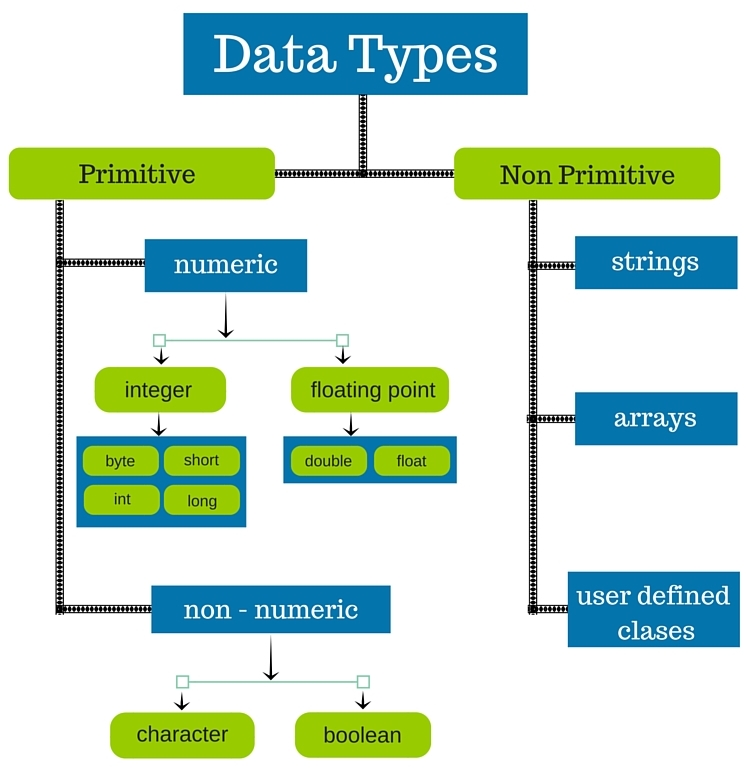
\includegraphics[scale=0.35]{Images/chapter02_section_04_primitive.jpg}
    \end{figure}
\end{frame}

\begin{frame}[fragile]{Primitive Data Types}
    \noindent
    \begin{figure}[H]
    \centering
    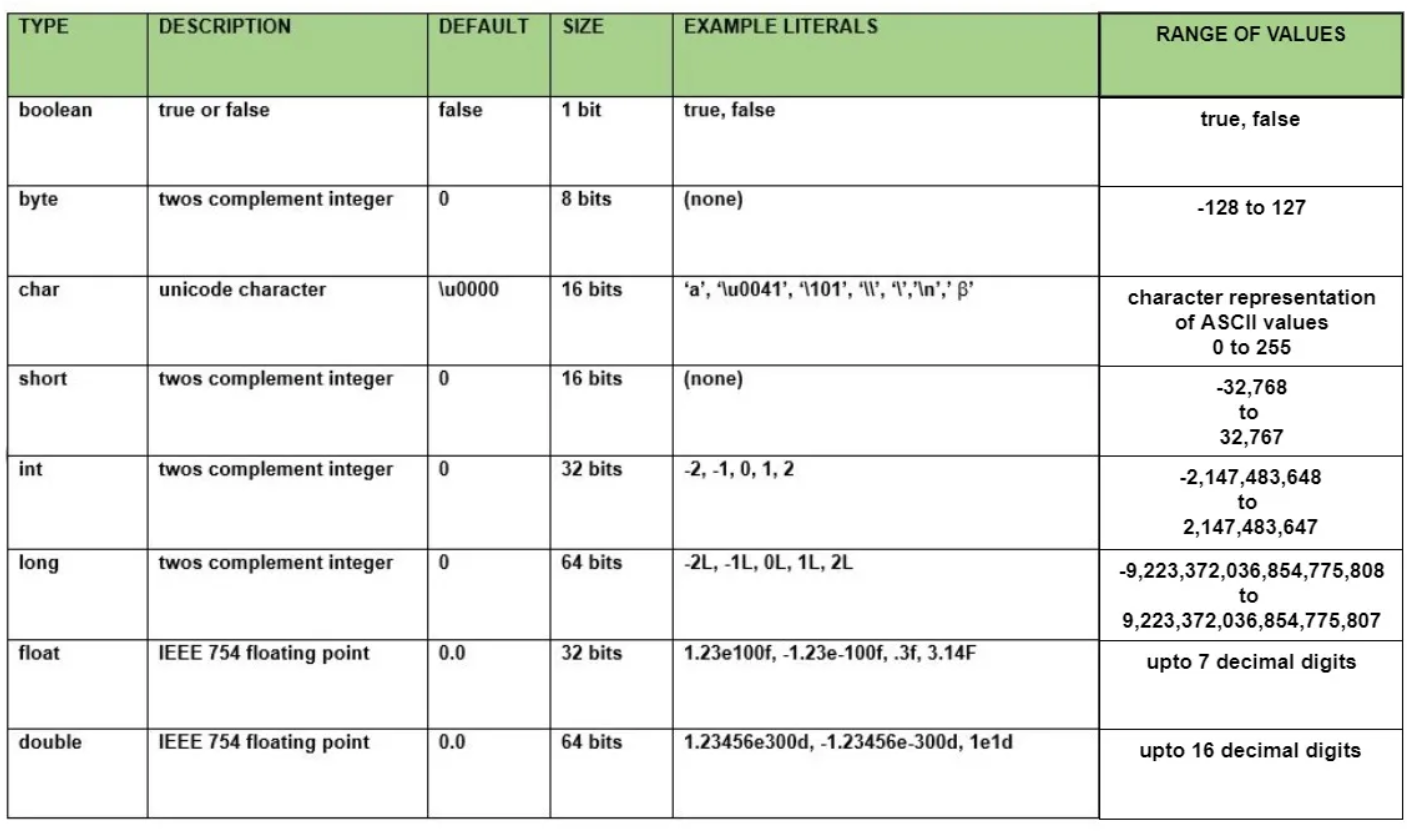
\includegraphics[scale=0.35]{Images/chapter02_section04_primitive01.png}
    \end{figure}
\end{frame}

\begin{frame}[fragile]{Primitive Data Types}
    Variable declarations take the form
    \begin{lstlisting}
    DataType VariableName;
    \end{lstlisting}
    Examples:
    \begin{lstlisting}
    byte inches;
    int speed;
    short month;
    float sales_commission;
    double distance;
    \end{lstlisting}
    Note: These data types are called ``primitive'' because you cannot use them to create objects.
\end{frame}

\begin{frame}[fragile]{Primitive Data Types}
    You cannot embed commas in \violet{numeric literals}.
    \begin{lstlisting}
    number = 1,257,649; // error
    number = 1257649; // correct
    \end{lstlisting}
    Floating point \violet{literals} are assumed to be of the \texttt{double} data type. Be careful assigning floating-point literals to a \texttt{float} variable.
    \begin{lstlisting}
        float number;
        number = 23.5; // error
    \end{lstlisting}
    This is because a \texttt{double} value is not compatible with \texttt{float} variable. A fix is
    \begin{lstlisting}
        float number;
        number = 23.5F;
    \end{lstlisting}
\end{frame}

\begin{frame}[fragile]{Primitive Data Types}
    A value is put into a \violet{variable} with an assignment statement. \\ \vspace{1em}
    For example, the following statement assigns the value 12 to the \violet{variable} \texttt{units\_sold}:
    \begin{lstlisting}
    units_sold = 12;
    \end{lstlisting}
    The \red{$=$} symbol is called the \red{assignment operator}. \\ \vspace{1em}
    The operand on the left side of the $=$ operator must be a variable name. \\ \vspace{1em}
    The value on the right side of the $=$ symbol must be an expression that has a value.
\end{frame}

\begin{frame}[fragile]{Primitive Data Types}
    A \violet{variable} can hold only one value at a time. \\ \vspace{1em}
    When you assign a new value to a variable, the new value takes the place of the variable's previous contents.
    \begin{lstlisting}
    int x = 5;
    System.out.println(x);
    x = 99;
    System.out.println(x);
    \end{lstlisting}
\end{frame}

\section{Operators and Conversion Between Data Types}
\subsection{Arithmetic Operators}
\begin{frame}[fragile]{Arithmetic Operators}
    There are many operators for manipulating numeric values and performing arithmetic operations. \\ \vspace{1em}
    Generally, there are three types of operators: unary, binary, and ternary. We mostly work with unary and binary operators.
    \begin{lstlisting}
    negation_result = -5; // unary operator: -
    addition_result = 5 + 1; // binary operator: +
    mult_result = 5 * 2; // binary operator: *
    remainder_result = 17 % 3; // binary operator: %
    \end{lstlisting}
\end{frame}

\begin{frame}[fragile]{Arithmetic Operators}
    When both operands of the division operator are integers, the operator will perform integer division. \\ \vspace{1em}
    This means the result of the division will be an integer as well. \\ \vspace{1em}
    If there is a remainder, it will be discarded.
    \begin{lstlisting}
    double number;
    number = 5 / 2; // value of 2 is assigned to _number_
    number = 5.0 / 2; // value of 2.5 is assigned to _number_
    \end{lstlisting}
\end{frame}

\begin{frame}[fragile]{Arithmetic Operators}
    The Java API provides a class named \texttt{Math}, which contains numerous methods that are useful for performing complex mathematical operations. \\ \vspace{1em}
    We will briefly look at the \texttt{Math.pow} and \texttt{Math.sqrt} methods.
    \begin{lstlisting}
    result_01 = Math.pow(4.0, 2.0); // 4 ^ 2 = 16
    result_02 = 3 * Math.pow(6.0, 3.0); // 3 * 6 ^ 3 = 648
    result_03 = Math.sqrt(9.0); // (9) ^ (1 / 2) = 3
    \end{lstlisting}
\end{frame}

\subsection{Conversion Between Primitive Data Types}
\begin{frame}[fragile]{Conversion Between Primitive Data Types}
    Before a value can be stored in a variable, the value's data type must be compatible with the variable's data type. \\ \vspace{1em}
    Java performs some conversions between data types automatically, but does not automatically perform any conversion that can result in the loss of data.
\end{frame}

\begin{frame}[fragile]{Conversion Between Primitive Data Types}
    Java is a \texttt{strongly typed} language. \\ \vspace{1em}
    To assign a value to a variable Java checks the data types of the variable and the value being assigned to it to determine whether they are compatible.
    \begin{lstlisting}
    // narrowing conversion
    int x;
    double y = 2.5;
    x = y; // error: possible loss of precision
    \end{lstlisting}

    \begin{lstlisting}
    // widening conversion
    int x;
    short y = 2;
    x = y; // works with no issues
    \end{lstlisting}
\end{frame}

\begin{frame}[fragile]{Conversion Between Primitive Data Types}
    The \texttt{cast} operator lets you manually convert a value, even if it means that a
    narrowing conversion will take place. \\ \vspace{1em}
    Here is an example
    \begin{lstlisting}
    double number = 1.1;
    x = (int)number;
    \end{lstlisting}
\end{frame}

\section{\texttt{final}, Strings, and Scope}
\subsection{Named Constants with \texttt{final}}
\begin{frame}[fragile]{Named Constants with \texttt{final}}
    The final key word can be used in a variable declaration to make the variable a named constant. \\ \vspace{1em}
    Named constants are initialized with a value, and that value cannot change during the execution of the program.
    \begin{lstlisting}
double interest_rate = 0.069; // initial value of interest_rate
interest_rate = 0.01; // interest_rate has now changed
final double INTEREST_RATE = 0.069; // cannot modify
INTEREST_RATE = 0.01; // error
    \end{lstlisting}
\end{frame}

\subsection{The \texttt{String} Class}
\begin{frame}[fragile]{The \texttt{String} Class}
    We can think of strings as a sequence of characters. \\ \vspace{1em}
    The \texttt{String} class allows you to create \violet{objects} for holding strings. \\ \vspace{1em}
    It also has various methods that allow you to work with strings. \\ \vspace{1em}
     It can be used to represent any type of data that contains text, such as names, addresses, warning messages, and so forth. \\ \vspace{1em}
     String literals are enclosed in double-quotation marks, such as the following:
     \begin{lstlisting}
    "Hello World"
    "Joe Mahoney"
     \end{lstlisting}
\end{frame}

\begin{frame}[fragile]{The \texttt{String} Class}
    The \violet{class} that is provided by the Java API for handling strings is named \texttt{String}. \\ \vspace{1em}
    To declare a variable of the \texttt{String} data type we can write the following:
    \begin{lstlisting}
    String string_variable_name;
    \end{lstlisting}
    The previous statement declares \texttt{string\_variable\_name} as a \texttt{String} variable. \\ \vspace{1em}
    Note that \texttt{String} is a \violet{class} not a \violet{primitive data type}.
\end{frame}

\begin{frame}[fragile]{Words of Wisdom}
    A variable of any type can be associated with an item of data. \\ \vspace{1em}
    A \violet{primitive type variable} holds the actual data item it is associated with. \\ \vspace{1em}
    A \violet{class type variable} does not hold the actual data item that it is associated with. \\ \vspace{1em}
    A \violet{class type variable} holds the memory address of the data item it is associated with. \\ \vspace{1em}
    \begin{lstlisting}
// The variable "number" holds the actual data
int number = 25;
// The variable "string_var" holds a reference to the data
String string_var = "pokemon";
    \end{lstlisting}
\end{frame}

\begin{frame}[fragile]{The \texttt{String} Class}
    Any time you write a string literal in your program, Java will create a \violet{String object} in memory to hold it. \\ \vspace{1em}
    You can create a \violet{String object} in memory and store its address in a \violet{String variable} with a simple assignment statement.
    \begin{lstlisting}
String name = "Joe Mahoney";
    \end{lstlisting}
    The \violet{string literal} causes a \violet{String object} to be created in memory with the value ``Joe Mahoney'' stored in it. \\ \vspace{1em}
    The assignment operator stores the address of that object in the \texttt{name} variable.
\end{frame}

\begin{frame}[fragile]{The \texttt{String} Class}
    Because the \texttt{String} type is a \violet{class}, it provides numerous \violet{methods} for working with strings.
    \begin{lstlisting}
    String fruit_name = "apple";
    int string_size;
    string_size = fruit_name.length();
    System.out.print(string_size); // prints "5"
    \end{lstlisting}
    Other methods in the \texttt{String} class are: \texttt{charAt(index), length(), toLowerCase(), toUpperCase()}.
\end{frame}

\subsection{Scope}
\begin{frame}[fragile]{Scope}
    A variable's \violet{scope} is the part of the program that has access to the variable. \\ \vspace{1em}
    Every variable has a scope. \\ \vspace{1em}
    The scope of a variable is the part of the program where the variable may be accessed by its name. \\ \vspace{1em}
    Variables that are declared inside a method are called \texttt{local variables}.
    \begin{lstlisting}
    public class ScopeExample {
        public static void main(String[] args) {
            int value = 100; // example of a local variable
            }
        }
    \end{lstlisting}
\end{frame}

\begin{frame}[fragile]{Scope}
    A local variable's scope begins at the variable's declaration and ends at the end of the method in which the variable is declared. \\ \vspace{1em}
    Here is an example of calling a variable outside of its scope.
    \begin{lstlisting}
    public class ScopeExample {
        public static void main(String[] args) {
            System.out.println(value); // error
            int value = 100;
            }
        }
    \end{lstlisting}
\end{frame}

\section{Comments, Style, and Keyboard Input}
\subsection{Comments}
\begin{frame}[fragile]{Comments}
    Comments are notes of explanation that document lines or sections of a program. \\ \vspace{1em}
    Comments are part of the program, but the compiler ignores them. \\ \vspace{1em}
    They are intended for people who may be reading the source code. \\ \vspace{1em}
    There are three types of comments: \red{single-line comments}, \red{multiline comments}, and \red{documentation comments}.
\end{frame}

\begin{frame}[fragile]{Comments}
    Let's see an example of single-line comments.
\begin{lstlisting}
// CommentSingleLine.java
public class CommentSingleLine {
    public static void main(String[] args) {
        double x = 10; // Define var x and assign value of 10
        double y = 5; // Define var y and assign value of 5
        double z; // Define var z
        z = x + y; // Assign sum of 10 and 5 to z
        }
    }
\end{lstlisting}
\end{frame}

\begin{frame}[fragile]{Comments}
    Now, a multi-line example.
\begin{lstlisting}
/*
    PROGRAM: CommentMultiLine.java
    Written by Jesus Perez Cuarenta
    This program shows how to add two doubles in Java.
*/
public class CommentMultiLine {
    public static void main(String[] args) {
        double x = 10;
        double y = 5;
        double z;
        z = x + y;
        }
    }
\end{lstlisting}
\end{frame}

\begin{frame}[fragile]{Comments}
    Finally, documentation comments. \\ \vspace{1em}
    These can be read and processed by a program named \texttt{javadoc}, which comes with the JDK. \\ \vspace{1em}
    If the source code files contain any documentation comments, the information in the comments becomes part of the HTML documentation. \\ \vspace{1em}
    The HTML documentation files may be viewed in a Web browser. \\ \vspace{1em}
    \red{Any comment that starts with \slash{}** and ends with *\slash{} is considered a documentation comment.}
\end{frame}

\begin{frame}[fragile]{Comments}
    \begin{lstlisting}
/**
    This class crates a program that adds two numbers of type double.
*/
public class CommentDocumentation {
    /**
        The main method is the program's starting point.
    */
    public static void main(String[] args) {
        double x = 10;
        double y = 5;
        double z = x + y;
        }
    }
    \end{lstlisting}
\end{frame}

\begin{frame}[fragile]{Comments}
    You can run the \texttt{javadoc} program from the operating system command prompt. \\ \vspace{1em}
    The general form is
\begin{lstlisting}
javadoc SourceFile.java
\end{lstlisting}
    For our example, we would type
\begin{lstlisting}
javadoc CommentDocumentation.java
\end{lstlisting}
\end{frame}

\subsection{Programming Style}
\begin{frame}[fragile]{Programming Style}
    Programming style refers to the way a programmer uses spaces, indentations, blank lines, and punctuation characters to visually arrange a program's source code. \\ \vspace{1em}
    The compiler doesn't care that each statement is on a separate line, or that spaces separate operators from operands. \\ \vspace{1em}
    Humans find it difficult to read programs that aren't written in a visually pleasing manner.
\end{frame}

\begin{frame}[fragile]{Programming Style}
    What to avoid:
    \begin{lstlisting}
// Compact.java
public class Compact {public static void main(String[] args) {int
    shares=220; double averagePrice=14.67; System.out.println(
    "There were "+shares+" shares sold at $"+averagePrice+
    " per share.");}}
    \end{lstlisting}
\end{frame}

\begin{frame}[fragile]{Programming Style}
    Instead, follow:
    \begin{lstlisting}
public class Readable {
    public static void main(String[] args) {
        int shares = 220;
        double averagePrice = 14.67;
        System.out.println(
            "There were " + shares
            + " shares sold at $"
            + averagePrice + " per share."
            );
        }
    }
    \end{lstlisting}
\end{frame}

\subsection{Reading Keyboard Input}
\begin{frame}[fragile]{Reading Keyboard Input}
    Recall that the \texttt{System.out} object refers to the standard output device. \\ \vspace{1em}
    The Java API has another object: \texttt{System.in}, which refers to the standard input device. \\ \vspace{1em}
    The \texttt{System.in} object reads input only as \texttt{byte} values. \\ \vspace{1em}
    We typically read keystrokes using \texttt{System.in} in conjunction with an object from the \texttt{Scanner} class.
\end{frame}

\begin{frame}[fragile]{Reading Keyboard Input}
    Here is a snippet that can be included inside the \texttt{main} method in a Java program:
\begin{lstlisting}
int number;
Scanner keyboard = new Scanner(System.in);
System.out.print("Enter an integer value: ");
number = keyboard.nextInt();
System.out.println(number);
\end{lstlisting}
Note that the \texttt{nextInt} method formats an input value as an \texttt{int} which jives with the definition of the \texttt{number} variable.
\end{frame}

\begin{frame}[fragile]{Reading Keyboard Input}
    The \texttt{Scanner} class contains more methods similar to \texttt{nextInt} such as
    \begin{itemize}
        \item \texttt{nextByte}
        \item \texttt{nextDouble}
        \item \texttt{nextFloat}
        \item \texttt{nextInt}
        \item \texttt{nextLine}
        \item \texttt{nextLong}
        \item \texttt{nextShort}
    \end{itemize}
\end{frame}

\begin{frame}[fragile]{Reading Keyboard Input}
    The \texttt{Scanner} class is not automatically available to your Java program. \\ \vspace{1em}
    Any program that uses the \texttt{Scanner} class should have the following statement near the beginning of the file, before any class definition:
    \begin{lstlisting}
import java.util.Scanner;
    \end{lstlisting}
This statement tells the Java compiler where in the Java library to find the \texttt{Scanner} class, and makes it available to your program.
\end{frame}

\end{document}

